%%%%%%%%%%%%%%%%%%%%%%%%%%%%%%%%%%%%%%%%%%%%%%%%%%%%%%%%%%%%%%%%%%%%%%%%
% Escuela Politécnica Superior de la Universidad de Alicante
% Realizado por: Jose Manuel Requena Plens
% Contacto: info@jmrplens.com / Telegram:@jmrplens
%%%%%%%%%%%%%%%%%%%%%%%%%%%%%%%%%%%%%%%%%%%%%%%%%%%%%%%%%%%%%%%%%%%%%%%%

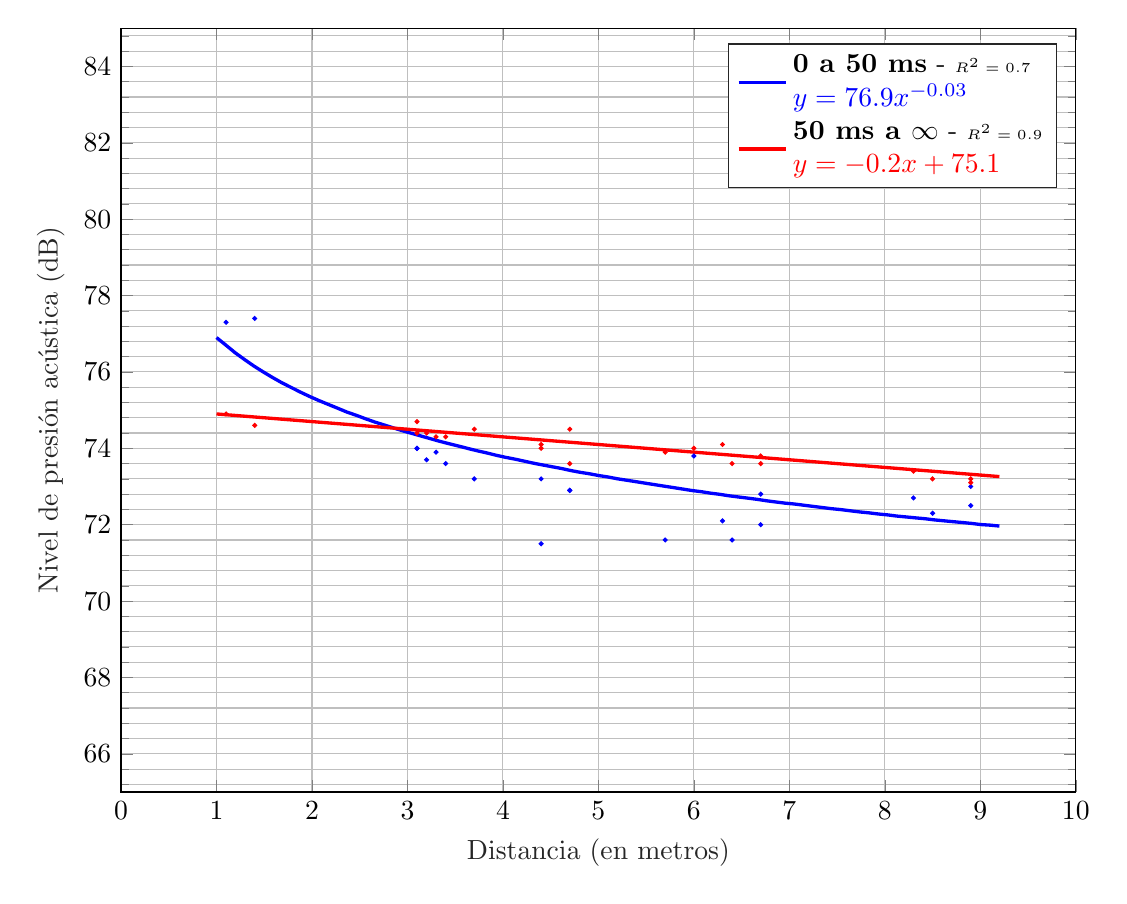
\begin{tikzpicture}

\begin{axis}[%
width=\textwidth,
height=0.8\textwidth,
at={(0\textwidth,0\textwidth)},
scale only axis,
xmin=0,
xmax=10,
xlabel style={font=\color{white!15!black}},
xlabel={Distancia (en metros)},
ymin=65,
ymax=85,
xmajorgrids,
xminorgrids,
ymajorgrids,
yminorgrids,
minor y tick num= 4,
ylabel style={font=\color{white!15!black}},
ylabel={Nivel de presión acústica (dB)},
axis background/.style={fill=white},
%xmajorgrids,
%xminorgrids,
%ymajorgrids,
%yminorgrids,
legend style={legend cell align=left, align=left, draw=white!15!black}
]
\addplot[color=blue,domain=1:9.2, samples=85,line width=1.2]{76.9*x^(-0.03)};
\addlegendentry{\textbf{0 a 50 ms} - \tiny{$R^2 = 0.7$}\\$\color{blue}y = 76.9·x^{-0.03}$}

\addplot[color=red,domain=1:9.2, samples=85,line width=1.2]{-0.20*x+75.10};
\addlegendentry{\textbf{50 ms a $\infty$} - \tiny{$R^2 = 0.9$}\\$\color{red}y = -0.2·x+75.1$}

% Puntos
\addplot [color=blue, only marks,mark size=0.7pt]
  table[row sep=crcr]{%
  8.9	72.5\\
6.7	72.0\\
4.7	72.9\\
3.3	73.9\\
3.1	74.0\\
4.4	73.2\\
6.4	71.6\\
8.3	72.7\\
6.0	73.8\\
3.7	73.2\\
1.4	77.4\\
1.1	77.3\\
3.4	73.6\\
5.7	71.6\\
8.9	73.0\\
6.7	72.8\\
4.7	72.9\\
3.2	73.7\\
3.1	74.0\\
4.4	71.5\\
6.3	72.1\\
8.5	72.3\\
  };
  
  \addplot [color=red, only marks,mark size=0.7pt]
  table[row sep=crcr]{%
  8.9	73.2\\
6.7	73.8\\
4.7	74.5\\
3.3	74.3\\
3.1	74.7\\
4.4	74.1\\
6.4	73.6\\
8.3	73.4\\
6.0	74.0\\
3.7	74.5\\
1.4	74.6\\
1.1	74.9\\
3.4	74.3\\
5.7	73.9\\
8.9	73.1\\
6.7	73.6\\
4.7	73.6\\
3.2	74.4\\
3.1	74.4\\
4.4	74.0\\
6.3	74.1\\
8.5	73.2\\
  };
\end{axis}
\end{tikzpicture}%